\begin{figure}[h]
    \centering
    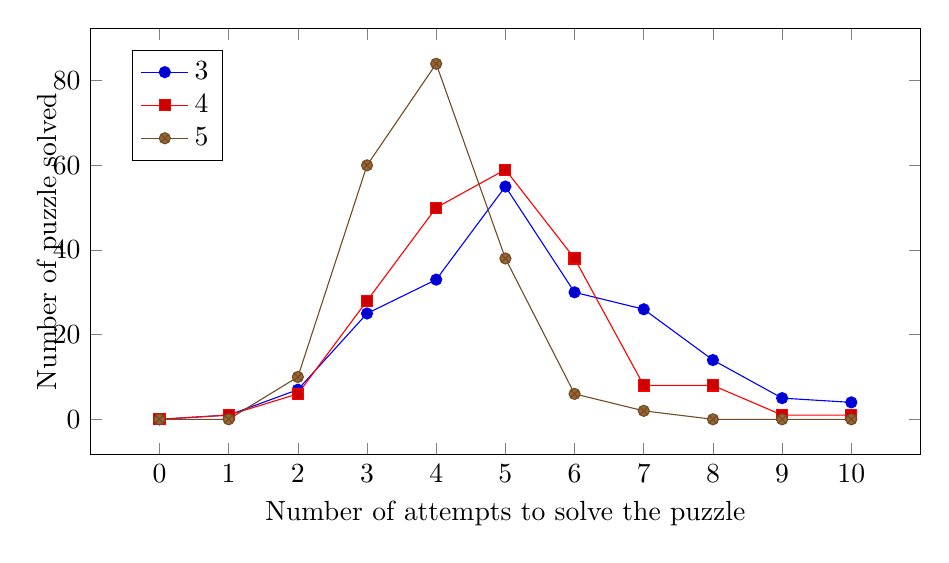
\begin{tikzpicture}
        \begin{axis}[
            xlabel=Number of attempts to solve the puzzle,
            width=\linewidth,
            height=7cm,
            ylabel=Number of puzzle solved,
            ylabel style={yshift=-10pt},
            xtick=data,
            legend style={at={(0.05,0.95)},anchor=north west}
            ]
        \addplot
            coordinates {
                (0, 0)
                (1, 1)
                (2, 7)
                (3, 25)
                (4, 33)
                (5, 55)
                (6, 30)
                (7, 26)
                (8, 14)
                (9, 5)
                (10, 4)
                };
        \addplot
            coordinates {
                (0, 0)
                (1, 1)
                (2, 6)
                (3, 28)
                (4, 50)
                (5, 59)
                (6, 38)
                (7, 8)
                (8, 8)
                (9, 1)
                (10, 1)
                };
            \addplot
            coordinates {
                (0, 0)
                (1, 0)
                (2, 10)
                (3, 60)
                (4, 84)
                (5, 38)
                (6, 6)
                (7, 2)
                (8, 0)
                (9, 0)
                (10, 0)
                };
                       
        \legend{3, 4, 5} 
        \end{axis}
    \end{tikzpicture}
    \caption{Automatic guesser performances measures}
\end{figure}